\documentclass{article}
\usepackage{tikz}

\begin{document}

% TikZ Coordinate Systems Demo
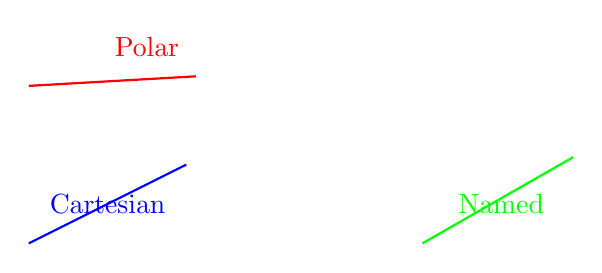
\begin{tikzpicture}[scale=1]

  % --- Cartesian coordinates (x,y) ---
  \draw[thick, blue] (0,0) -- (2,1);
  \node[blue] at (1,0.5) {Cartesian};

  % --- Polar coordinates (angle:radius) ---
  \draw[thick, red] (90:2) -- (45:3);
  \node[red] at (1.5,2.5) {Polar};

  % --- Named coordinates (A, B) ---
  \coordinate (A) at (5,0);
  \coordinate (B) at (9:7);
  
  \draw[thick, green] (A) -- (B);
  \node[green] at (6,0.5) {Named};

\end{tikzpicture}

\end{document}
